Data analysis in the context of this project is completed as a series of stages, each of which consists of a sequential process of ETL, followed by querying and analysis. Figure \ref{analysis-workflow} shows the sequential steps involved in a single stage of analysis; nETL is executed with a configuration file specifying CSV extraction, transformations, and the destination database as a parameter, CouchDB builds a view-index according to the MapReduce view as specified via a design document, data is retrieved via a List function also specified on the design document, and subsequent analyses (stages) are performed in context of the proceeding stages results. For each stage in the analysis, the configuration of nETL is discussed in terms of logical operations, and the configuration files themselves are included in the appendix (see \ref{netl-configuration}).

With the eventual aim of assessing the relationships between LMS usage and course grades, the following series of analyses is conducted in terms of the CSC1015F course.

\begin{enumerate}
    \item \textit{Stage 1}: Assessing effectiveness of different benchmarking formulas using the Benchmarks data
    \item \textit{Stage 2}: Assessing the correlation between Events and Grades data
    \item \textit{Stage 3}: As a means of control, assessing the correlation between Events and Benchmarks
    \item \textit{Stage 4}: Assessing the relationship of student performance relative to their peers as benchmarked compared to course performance, in terms of LMS usage
\end{enumerate}
\begin{figure}[]
    \centering
    \begin{mdframed}
        \centering
        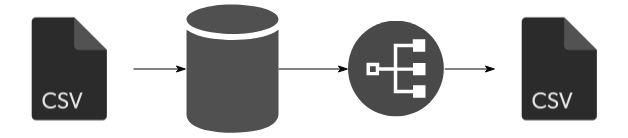
\includegraphics[scale=0.35]{./resources/figures/analysis.png}
    \end{mdframed}
    \caption[Analysis Workflow]{\textbf{Figure \ref{analysis}: Workflow to perform an analysis.} The analysis process represented as a simple pipeline. First nETL extracts data from CSV files and loads that into a CouchDB database via the CouchDB server API. This file consists of a B+tree organized by the \_id field of each document created as a UUID on document write by CouchDB to guarantee uniqueness of every document. From the database file an index is created, also structured as a B+tree but organized by a key as a specified in the Map Function. This allows for sorted output according to a users requirements. A List function is used to retrieve the contents of the view, transform those contents into tabular (CSV) form. The result of calling the List function is a downloaded CSV file. The List function address (API) is of the form \texttt{http(s)://<host>:<port>/<db>/\_design/<doc>/\_list/<fn>/<view>?<params>}}
    \label{analysis}
\end{figure}

In addition to outlining a structured approach by which the results are obtained for CSC1015F, further discussion is provided on how multiple courses may be analyzed simultaneously via more advanced usage of CouchDB's MapReduce implementation. During analysis, runtime results of the different components of the system are recorded and are shown in Table \ref{performance-analysis}. The metrics include running time of nETL tasks, a summary of the data processed by nETL, CouchDB indexing times, and database/index storage footprints.

In terms of defining MapReduce tasks, the map function is always user-defined, whereas a built-in reduce function (\_stats) is always used. The built-in reduce function are implemented within the main Erlang process, which according to the documentation offers a performance boost since the IO transfer cost between the Erlang process and the view engine (couchjs.exe by default) is negated. Working on a Windows machine the IO cost is apparently exaggerated (see the slack correspondence with Jan Lehnardt in appendix \ref{slack-1-nov}) due to the difference between Unix-based and Windows kernel implementations.

\begin{table}[H]
    \begin{threeparttable}
        \textbf{Table \ref{tbl-grades-normalize}}\par\medskip\par\medskip
        \caption{Grade results need to be treated as numbers for the purpose of this analysis, this table shows all different value types and the appropriate treatment for each. Because of the volume of data, it was not checked how many of these symbols apply to undergraduate students specifically, so these cases were handled generically}
        \label{tbl-grades-normalize}
        \begin{tabularx}{\textwidth}{>{\hsize=0.6\hsize}X>{\hsize=1.3\hsize}X>{\hsize=1.1\hsize}X}
            \toprule
            \mC{c}{Symbol} & \mC{c}{Meaning}          & \mC{c}{Handling Logic}                     \\
            \midrule
            49A            & Absent for supplementary & Grade used                                 \\
            49S            & Supplementary pending    & Grade used                                 \\
            50C            & ?                        & Grade used                                 \\
            78             & Grade                    & Grade used                                 \\
            AB             & Absent (fail)            & N/A                                        \\
            ATT            & ?                        & N/A                                        \\
            DE             & Deferred                 & N/A                                        \\
            DPR            & Duly performed refused   & 30\% Grade used\tnote{\textsuperscript{1}} \\
            F              & Fail                     & 40\% Grade used\tnote{\textsuperscript{2}} \\
            GIP            & Thesis only              & N/A                                        \\
            INC            & Incomplete (fail)        & 30\% Grade used\tnote{\textsuperscript{1}} \\
            LOA            & Leave of absence         & N/A                                        \\
            OS             & Outstanding              & N/A                                        \\
            OSS            & Outstanding              & N/A                                        \\
            PA             & Pass (thesis)            & N/A                                        \\
            SAT            & Thesis only              & N/A                                        \\
            UF             & Unclassified Fail        & 49\% Grade used\tnote{\textsuperscript{3}} \\
            UNS            & Thesis only              & N/A                                        \\
            UP             & Unclassified pass        & 45\% Grade used\tnote{\textsuperscript{4}} \\
            \bottomrule
        \end{tabularx}
        \scriptsize
        \begin{tablenotes}
            \item[\textsuperscript{1}]30\% was applied on the estimate that these students wouldn't necessarily have completed the coursework, and that as such this is a `bad' fail
            \item[\textsuperscript{2}]40\% was applied on the estimate that this symbol would apply to students who participated in the course but still failed
            \item[\textsuperscript{3}]49\% was applied on the estimate that this is a `good' fail, in that the UF classification applies to borderline fails
            \item[\textsuperscript{4}]45\% was applied on the estimate that UP is the 'worst' pass, in that from a strictly grade perspective, these students technically failed
        \end{tablenotes}
    \end{threeparttable}
\end{table}
\begin{table}[H]
    \begin{threeparttable}
        \textbf{Table \ref{performance-analysis}}\par\medskip\par\medskip
        \caption[Software performance analysis]{Running time analysis of \textit{nETL} tasks and CouchDB MapReduce indexing}
        \label{performance-analysis}
        \begin{tabularx}{\textwidth}{>{\hsize=1.8\hsize}X>{\hsize=0.8\hsize}Y>{\hsize=0.8\hsize}Y>{\hsize=0.8\hsize}Y>{\hsize=0.8\hsize}Y}
            \toprule
            \mC{c}{}                                               & \mC{c}{2-Way Join} & \mC{c}{3-Way-join}             & \mC{c}{Variance} & \mC{c}{Tests} \\
            \midrule
            Demographic lines extracted                            & -                  & -                              & -                &               \\
            Demographic lines loaded                               & -                  & -                              & -                &               \\
            Demographic task time (sec)\tnote{\textsuperscript{1}} & -                  & -                              & -                &               \\
            \midrule
            Grade lines extracted                                  & -                  & -                              & -                &               \\
            Grade lines loaded                                     & -                  & -                              & -                &               \\
            Grade task time (sec)\tnote{\textsuperscript{1}}       & -                  & -                              & -                &               \\
            \midrule
            Events lines extracted                                 & -                  & 44 420 508                     &                  &               \\
            Events lines loaded                                    & -                  & -                              & -                &               \\
            Events task time (sec)\tnote{\textsuperscript{1}}      & -                  & -                              & -                &               \\
            \midrule
            CouchDB footprint (MB)\tnote{\textsuperscript{2}}      & -                  & -                              & -                &               \\
            View calculation time (sec)\tnote{\textsuperscript{3}} & -                  & -                              & -                &               \\
            View size (MB)                                         & -                  & -                              & -                &               \\
            \midrule
            List function output                                   & -                  & 586\tnote{\textsuperscript{4}} & -                & -             \\
            \bottomrule
        \end{tabularx}
        \scriptsize
        \begin{tablenotes}
            \item[\textsuperscript{1}]Tasks are run asynchronously, so time taken includes processing of other tasks in this run. Task run times are printed out to the log
            \item[\textsuperscript{2}]This is representative of the amount of data processed by \textit{nETL}
            \item[\textsuperscript{3}]CouchDB views are calculated per shard. By default a database contains 8 shards (even in single node mode). The log file shows start and end times of view calculations for each shard, the time is taken as time the first shard starts indexing, to the time the last shard stops indexing
            \item[\textsuperscript{4}]This file comprises a unique list of students, each student associated with the joined output.
        \end{tablenotes}
    \end{threeparttable}
\end{table}


todo:

Hi Sonia.

I’m looking at the two approaches to using MapReduce to aggregate data across different entities in CouchDB.

A bit about how view are produced in CouchDB:
CouchDB iterates through the docs, and runs the map function on every document, which the user configures to ‘emit’ values. For my function, the emitted value is a tuple with 11 indexes, with every value initialized at 0. So it’s this: [0,0,0,0,0,0,0,0,0,0,0]. Then depending on the document being processed by the map function, values at different indexes are changed.

i.e. if the document being processed by the map function is a ‘grade’ document, then the map function adjusts the value tuple to emit the grade percent – i.e. [percent, 0,0,0,0,0,0,0,0,0,0]. Or if the document is of type ‘demographic’, the map function changes the values at indexes 2 through 9 and emits the value: [0, x,x,x,x,x,x,x,x, 0, 0]. If the document is of type ‘event’, then the map function alters the value at indexes 9 and 10. i.e. [0,0,0,0,0,0,0,0, s1Event, s2Event] (s1Event is 1 for first semester event, or 0 for second semester, etc.).

And as you recommended, the keys are always emitted as [student id, course, year] for grade document, [student id, ‘a’, 1] for demographic documents, and [student id, ‘a’, year] for event documents.

But then I can never group the different document types for a student id. Instead I’m guaranteed that all documents for a single student are ‘next’ to each other and I can join them from iteration as a result. i.e. this is the result of the map function for a single student for 2 courses

    [smtzac002, ‘a’, 1]: [0, b1, b2, b3, b4, b5, b6, b7, b8, 0, 0]
[smtzac002, ‘a’, 2016]: [0, 0, 0, 0, 0, 0, 0, 0, 0, 1, 0]
[smtzac002, ‘a’, 2016]: [0, 0, 0, 0, 0, 0, 0, 0, 0, 1, 0]
[smtzac002, ‘a’, 2016]: [0, 0, 0, 0, 0, 0, 0, 0, 0, 0, 1]
[smtzac002, ‘a’, 2016]: [0, 0, 0, 0, 0, 0, 0, 0, 0, 0, 1]
[smtzac002, ‘a’, 2016]: [0, 0, 0, 0, 0, 0, 0, 0, 0, 0, 1]
[smtzac002, ‘a’, 2016]: [0, 0, 0, 0, 0, 0, 0, 0, 0, 1, 0]
[smtzac002, ‘CSC1015F’, 2016]: [98, 0, 0, 0, 0, 0, 0, 0, 0, 0, 0]
[smtzac002, ‘MAM100F, 2016]: [94, 0, 0, 0, 0, 0, 0, 0, 0, 0, 0]

Then the reduce function is only necessary to aggregate the event data (which will all have the same key). The result is something like this:

[smtzac002, ‘a’, 1]: [0, b1, b2, b3, b4, b5, b6, b7, b8, 0, 0]
[smtzac002, ‘a’, 2016]: [0, 0, 0, 0, 0, 0, 0, 0, 0, 3, 3]
[smtzac002, ‘CSC1015F’, 2016]: [98, 0, 0, 0, 0, 0, 0, 0, 0, 0, 0]
[smtzac002, ‘MAM100F, 2016]: [94, 0, 0, 0, 0, 0, 0, 0, 0, 0, 0]

(although the structure of the reduce output is a little different to this, the information is the same)

Then the actual aggregation is done on retrieval. So it would be better to do the actual aggregation in nETL then.

Is that ok? But this means that the importance of the reduce function is greatly diminished. So effectively I’m using CouchDB to order the information in the CSV, and nothing more really…

Alternatively, what I did was this:
[smtzac002, ‘x’, y]: [0, b1, b2, b3, b4, b5, b6, b7, b8, 0, 0] // this document is emitted twice: where x = CSC1015F, and then when x = MAM100F. y = 2016 (since only one year is analyzed)
[smtzac002, ‘x’, 2016]: [0, 0, 0, 0, 0, 0, 0, 0, 0, 1, 0] // emitted for x = CSC1015F and x = MAM100F
    [smtzac002, ‘x’, 2016]: [0, 0, 0, 0, 0, 0, 0, 0, 0, 1, 0] // emitted for x = CSC1015F and x = MAM100F
    [smtzac002, ‘x’, 2016]: [0, 0, 0, 0, 0, 0, 0, 0, 0, 0, 1] // emitted for x = CSC1015F and x = MAM100F
    [smtzac002, ‘x’, 2016]: [0, 0, 0, 0, 0, 0, 0, 0, 0, 0, 1] // emitted for x = CSC1015F and x = MAM100F
    [smtzac002, ‘x’, 2016]: [0, 0, 0, 0, 0, 0, 0, 0, 0, 0, 1] // emitted for x = CSC1015F and x = MAM100F
    [smtzac002, ‘x’, 2016]: [0, 0, 0, 0, 0, 0, 0, 0, 0, 1, 0] // emitted for x = CSC1015F and x = MAM100F
    [smtzac002, ‘CSC1015F’, 2016]: [98, 0, 0, 0, 0, 0, 0, 0, 0, 0, 0] // emitted once
    [smtzac002, ‘MAM100F, 2016]: [94, 0, 0, 0, 0, 0, 0, 0, 0, 0, 0] // emitted once


So then the result of the reduce function is an aggregation already. BUT. If I am analyzing 40 courses, then every single event is emitted 40 times. And if I were analyzing multiple years, then every event would be emitted 40 times for each year (so 120 times for 3 years). Obviously this is not scalable.

Should I include the fact that I tried this approach in the write up? It seems like more a mistake than anything else in hindsite. I would prefer to just write up the steps to creating a correct and concise result.
